% takto sa píše komentár

% dokumentclass určuje ako bude dokument sádzaný. Aké veľké budú okraje. Aké písmo sa použije. Ako sa budú písať názvy kapitol, sekcií atď. Mohol by som napísať len \documentclass{article} ale ak chcem zmeniť defaultné nastavenia napíšem \documentclass[11pt, a4paper]{article} aby veľkosť hlavného fontu bol 11pt a formát strany a4. Defaultné nastavenia sú 10pt a letterpaper. Pre dalšie nastavenia viď "Nie príliš strucný úvod do systému LATEX2"
\documentclass[11pt, a4paper]{article}

% aby sme mohli používať Slovenčinu. Na internete sú aj iné navody ako spojazniť Slovenčinu v Latexu. Mne fungoval tento, vám možno nemusí. Sú aj návody na internete, ktoré mne nefungovali.
\usepackage[utf8x]{inputenc}
\usepackage[slovak]{babel}

%tento package použijem aby som mohol písať matematické rovnice
\usepackage{amsmath}
%\usepackage{IEEEtrantools}

%tento package použijem aby mohli byť referencie stlačitelné. Taktiež ich spraví farebnými. To sa dá vypnút buď pomocou nastavení alebo potom tento package nepoužiť
\usepackage{hyperref}

%aby som mohol vkladať obrázky
\usepackage{graphicx}
\usepackage{float}



% takto dáme Latexu vedieť kto je autor dokumentu a ako sa dokument volá. To že som to napísal tu neznamená, že to bude vo výslednom texte aj použité.
\author{Mária Somorovská}
\title{Ako písať v \LaTeX u}

% Latex dokument začína príkazom \begin{document} a končí \end{document}. Všetko čo je pred \begin{document} sa do textu nenapíše. Je to len na načítanie knižníc a definovaní informácií o autoroch názve atď. \begin{document} je niečo ako main v C/C++
\begin{document}

% tu použijem to čo som definoval hore. Príkaz \maketitle napíše názov dokumentu, autora a dnešný dátum. To ako to spraví je nastavené v documentclass article.
\maketitle

% keďže chcem mať názov na samostatnej strane použijem príkaz \newpage
\newpage


\begin{abstract}
Toto je abstrakt môjho dokumentu kde vysvetlujem základy \LaTeX u. Čítať by sa mal zdrojový kód tohto dokumentu a nie výstup. Výstupné pdf je len na pochopenie, čo presne jednotlivé príkazy robia. 

Lorem ipsum dolor sit amet, consectetur adipiscing elit. Sed sit amet sem erat. Vestibulum non tellus porta, bibendum lorem non, tristique diam. Proin dolor lectus, fermentum ut auctor ut, laoreet vitae ipsum. Nam quis sapien vitae enim malesuada gravida in pulvinar urna. Mauris urna ipsum, lacinia et est ac, ullamcorper convallis lectus. Pellentesque laoreet erat id finibus malesuada. Morbi non egestas enim, id tempor sapien. Mauris id nunc vel nisi viverra tincidunt. Donec in justo vehicula, blandit ante at, placerat erat. Phasellus sed diam non augue posuere fermentum. Vestibulum vitae sem eu leo posuere maximus. Phasellus scelerisque dolor non dolor semper varius. 
\end{abstract}

% keďže chcem mať abstrakt na samostatnej strane použijem príkaz \newpage
\newpage

% napíše obsah. Aj spôsob akým štýlom napíše obsah je definovaný v documentclass article. Obsah generuje automaticky.
\tableofcontents

% keďže chcem mať obsah na samostatnej strane použijem príkaz \newpage
\newpage

% príkazom \section vytvoríme prvú sekciu. 
\section{Názov kapitoly, ktorý sa automaticky vygeneruje do obsahu}
Text prvej sekcie. To ako sa sekcie číslujú a či sa vôbec čislujú je nastavené v documentclass. Text je napísaný od okraja po okraj. Väčší    počet    medzier    medzi    slovami    je    vo    výslednom    súbore    ignorovaný.
Jeden
nový
riadok
je
mezdi
slovami
ignorovaný.
Ak chceme napísať nový riadok vieme to pomocou príkazu \newline alebo \\ Ak chceme napísať nový odsek, treba napísať dva nové riadky. 

Toto je už nový odsek. To ako sa napíše nový odsek, či sa dá medzi odsekmi medzera alebo aké veľké je odsadenie od začiatku riadku je definované v documentclass. Je aj veľa daľšich spôsobou ako prinútiť \LaTeX napísať medzeru, nový riadok ako rozdeliť príliš dlhé slovo atď.





Ak chceme napísať text iným štyýlom. Hrubý text, italic, zvýraznený text použijeme príkazy \emph{Text}, \textbf{Text},\texttt{Text}, \textrm{Text}, \textsf{Text}, \textsc{Text}.

Môžeme meniť aj veľkosť textu {\tiny Text}, {\scriptsize Text}, {\footnotesize	 Text}, {\small	 Text}, {\normalsize	 Text}, {\large	 Text}, {\Large	 Text}, {\LARGE	 Text}, {\huge	 Text}, {\Huge	 Text}

\begin{center}
Môžme meniť aj zarovnanie textu nastred
\end{center}

\begin{flushright}
Môžme meniť aj zarovnanie textu napravo
\end{flushright}

\begin{flushleft}
Môžme meniť aj zarovnanie textu naľavo
\end{flushleft}

Ak chceme zväčšiť medzeru medzi slovami pozužijeme \ medzera \quad vačšia medzera \qquad ešte väčšia medzera. Ľubovolne veľká medzera \hspace{1cm} Tu bude veľká horizontálna medzera.

Ak chceme zväčšiť medzeru medzi riadkami pozužijeme \vspace{1cm} \\ Tu bude veľká vertikálna medzera.

Príkaz \hfill doplní riadok. Viď výstup.

Príkaz

\vfill

doplní stranu. A spolu s newpage napíše paragraf na koniec strany.
\newpage

Očíslovaný zoznam
\begin{enumerate}
\item prvá vec
\item druhá vec
\end{enumerate}

\subsection{subsekcia}

\section{Ako písať rovnice}
Matematické rovnice v \LaTeX u sú veda sama o sebe. Rovnicu môžeme napísať do riadku pomocou $a=b$. Pri písaní matematických symbolov \LaTeX\ použije iný font. Aj keď v texte použijeme len premennú napr. $x$, dáme ju medzi doláre aby sa zmenil font. Vtedy je matematický text lepšie čitatelný.

Keď chceme napísať rovnicu vo vlastnom riadku je nato viac možností. Preto som nazačiatku includol package amsmath.

Rovnice sú automaticky očislované. Keď pridáme rovnicu pred túto, tak sa všetky automaticky prečíslujú. 

Klasická čislovaná rovnica
\begin{equation}
a = b + c
\end{equation}
Klasická nečislovaná rovnica
\begin{equation*}
a = b + c
\end{equation*}

Niekedy sa môže stať že sa mi rovnica nezmestí do riadku
\begin{equation}
a + b + c + d + e + f
+ g + h + i = j + k + l + m + n + o + p + r + s + t + u + v + w + x + y + z + 1 + 2 + 3 + 4 + 5  
\end{equation}
Vtedy môžem použiť multline. Pomocou znaku \\ určím, kde sa má rovnica rozdeliť. Celá rovnica bude mať len jedno číslo.
\begin{multline}
a + b + c + d + e + f
+ g + h + i = j + k + l + m + n + o + p + r + \\
s + t + u + v + w + x + y + z + 1 + 2 + 3 + 4 + 5  
\end{multline}

Keď chcem použiť viacero samostatných očíslovaných rovníc v jednej použijem
\begin{eqnarray}
a = b\\
a = b\\
a = b
\end{eqnarray}
Keby som použil viac equation tak by tam boli príliš veľke medzery
\begin{equation}
a = b
\end{equation}
\begin{equation}
a = b 
\end{equation}
\begin{equation}
a = b
\end{equation}
podobný efekt ako s multline sa dá dosiahnúť aj pomocou eqnarray ak prinútim \LaTeX\ aby nečisloval riadok pomocou nonumber
\begin{eqnarray}
a + b + c + d + e + f
+ g + h + i = j + k + l + m + n + o + p + r + \nonumber \\
s + t + u + v + w + x + y + z + 1 + 2 + 3 + 4 + 5  
\end{eqnarray}

Multline však v niektorých prípadoch dáva krajšie výsledky
\begin{multline}
a + b + c + d + e + f + 1 + 2 + 3 + 4 \\
+ g + h + i + j + k + l + 1 + 2 + 3 + 4\\
+ m + n + o + p + q + 1 + 2 + 3 + 4
\end{multline}
\begin{eqnarray}
a + b + c + d + e + f + 1 + 2 + 3 + 4  \nonumber\\
+ g + h + i + j + k + l + 1 + 2 + 3 + 4 \nonumber\\
+ m + n + o + p + q + 1 + 2 + 3 + 4
\end{eqnarray}

Keď mám viac rovníc s = môže sa stať, že sa mi rovnice nezarovnajú na =
\begin{eqnarray}
a = b + c + d + e + f  \\
 g + h = i + j + k + l  \\
 m + n + o = p + q + 1 
\end{eqnarray}
Vtedy môžem použiť \& (bez backslachu. Inak by som to nemohol napísať) na zarovnanie na daný znak
\begin{eqnarray}
a &=& b + c + d + e + f  \\
 g + h &=& i + j + k + l  \\
 m + n + o &=& p + q + 1 
\end{eqnarray}
Je to ako keby sa rovnica rozdelila do viacerých stĺpcou a \& určuje nový stĺpec. V jednom riadku môžu byť najviac dve \&. Všimnite si veľké medzery medzi rovná sa.

Existuje viacero matematických prostredí. Líšia sa v tom ako zarovnávajú rovnice, ako ich číslujú a čo všetko v nich môžeme robiť.
$\in$

\LaTeX\ by bol zbytočný keby sme v ňom nemohli pisať špeciálne matematické znaky. Grécka abeceda $\alpha \beta \gamma \Gamma \Delta$ atď. Horný index sa píše pomocou striešky $x^2$. Dolný index pomocou podtržovníka $x_i$. Môžeme použiť aj horný a dolný index naraz $x^2_i$. Ak chceme do horného/dolného indexu dať viaz znakov treba ich dať do krútených zátvoriek a poprípade ich rôzne kombinovať $x^{2+3}_{i,j_k}$.

Integrál $\int_{lower}^{upper}$. Suma $\sum_{n=1}^{\infty} 2^{-n} = 1$ atď. Niektoré dobré \LaTeX\ editory majú tlačítka na pridávanie špeciálnych znakov. Je dobré si základné znaky pamätať.

\section{Obrázky}
Aj obrázky v \LaTeX u sú veda sama o sebe. Hlavne to kde ich \LaTeX\ vloží. Pomocou figure dám vedieť, že ide o obrázok. centering spôsobí, že obrázok bude v strede strany. Inak by bol nalavo ako text. Do includegraphics dám názov obrázka, ktorý tam má vložiť. Môžem ho napísať bez koncovky alebo s ňou. Obrázok sa musí nachádzat v adresáry, kde je zdrojový kód. Alebo k nemu môžem napísať cestu.
\begin{figure}
  \centering
      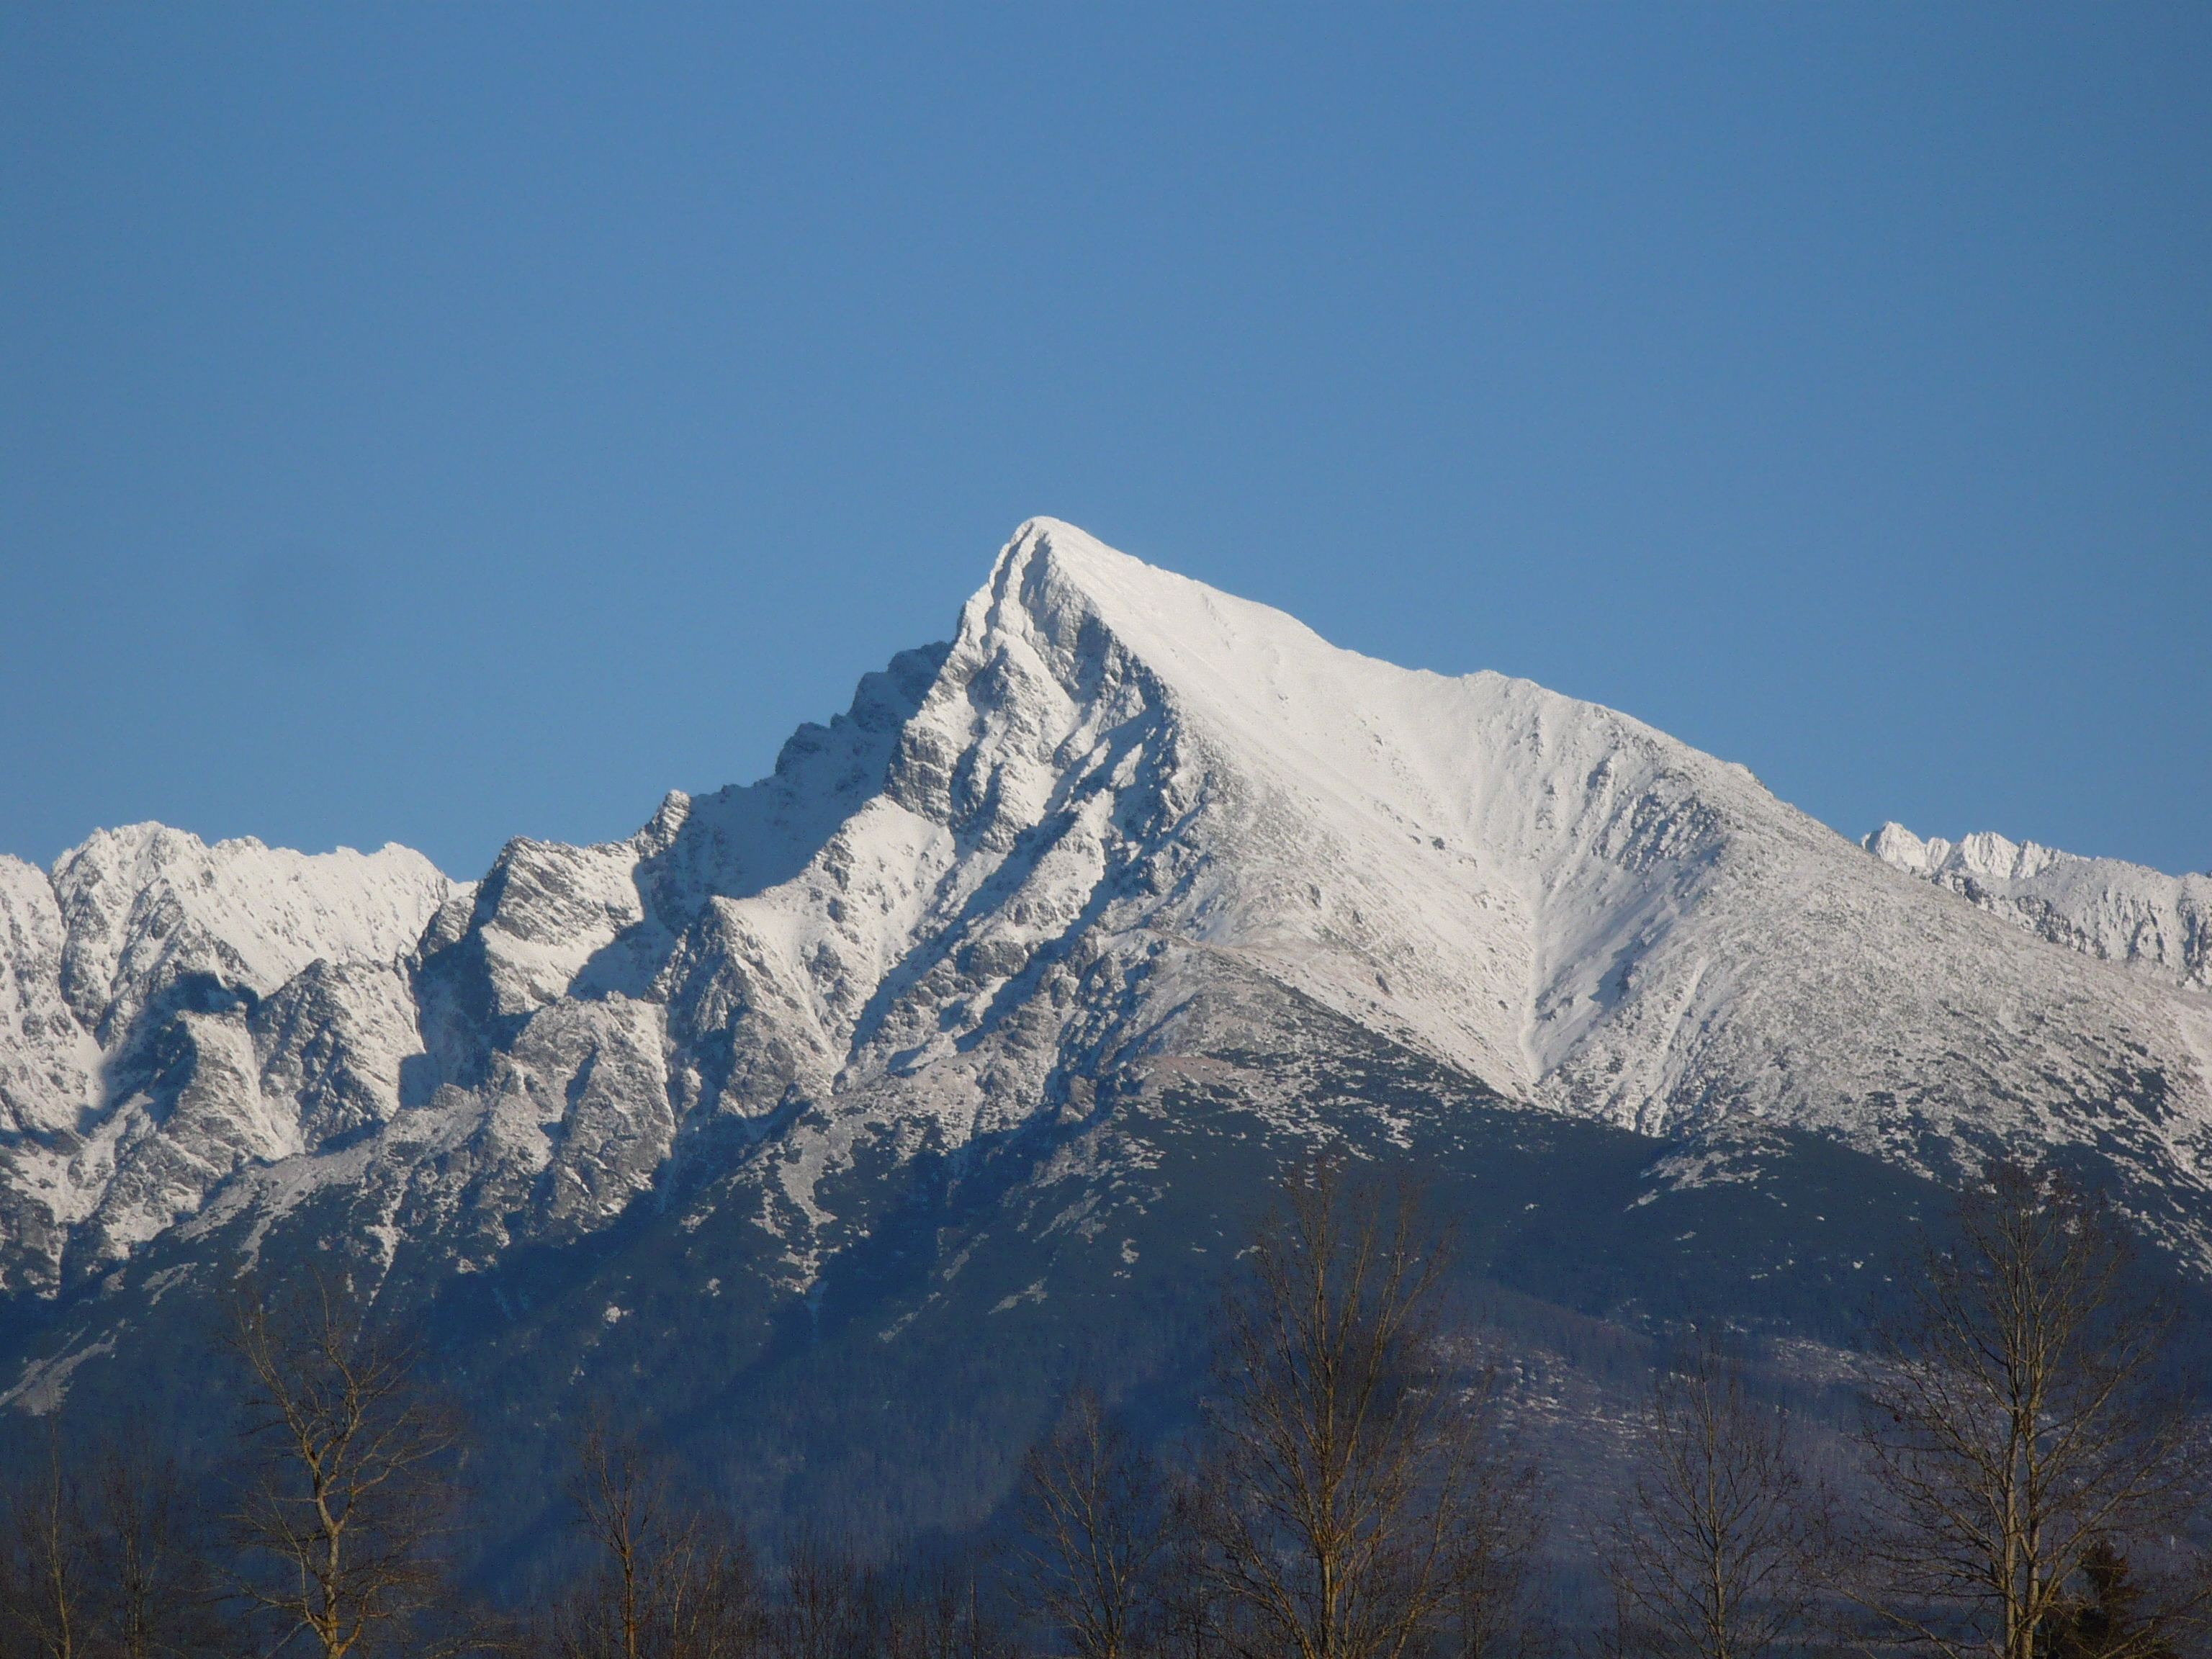
\includegraphics{krivan}
\end{figure}

Obrázok je priveľký. To sa dá zmeniť pomocou argumentu width
\begin{figure}
  \centering
      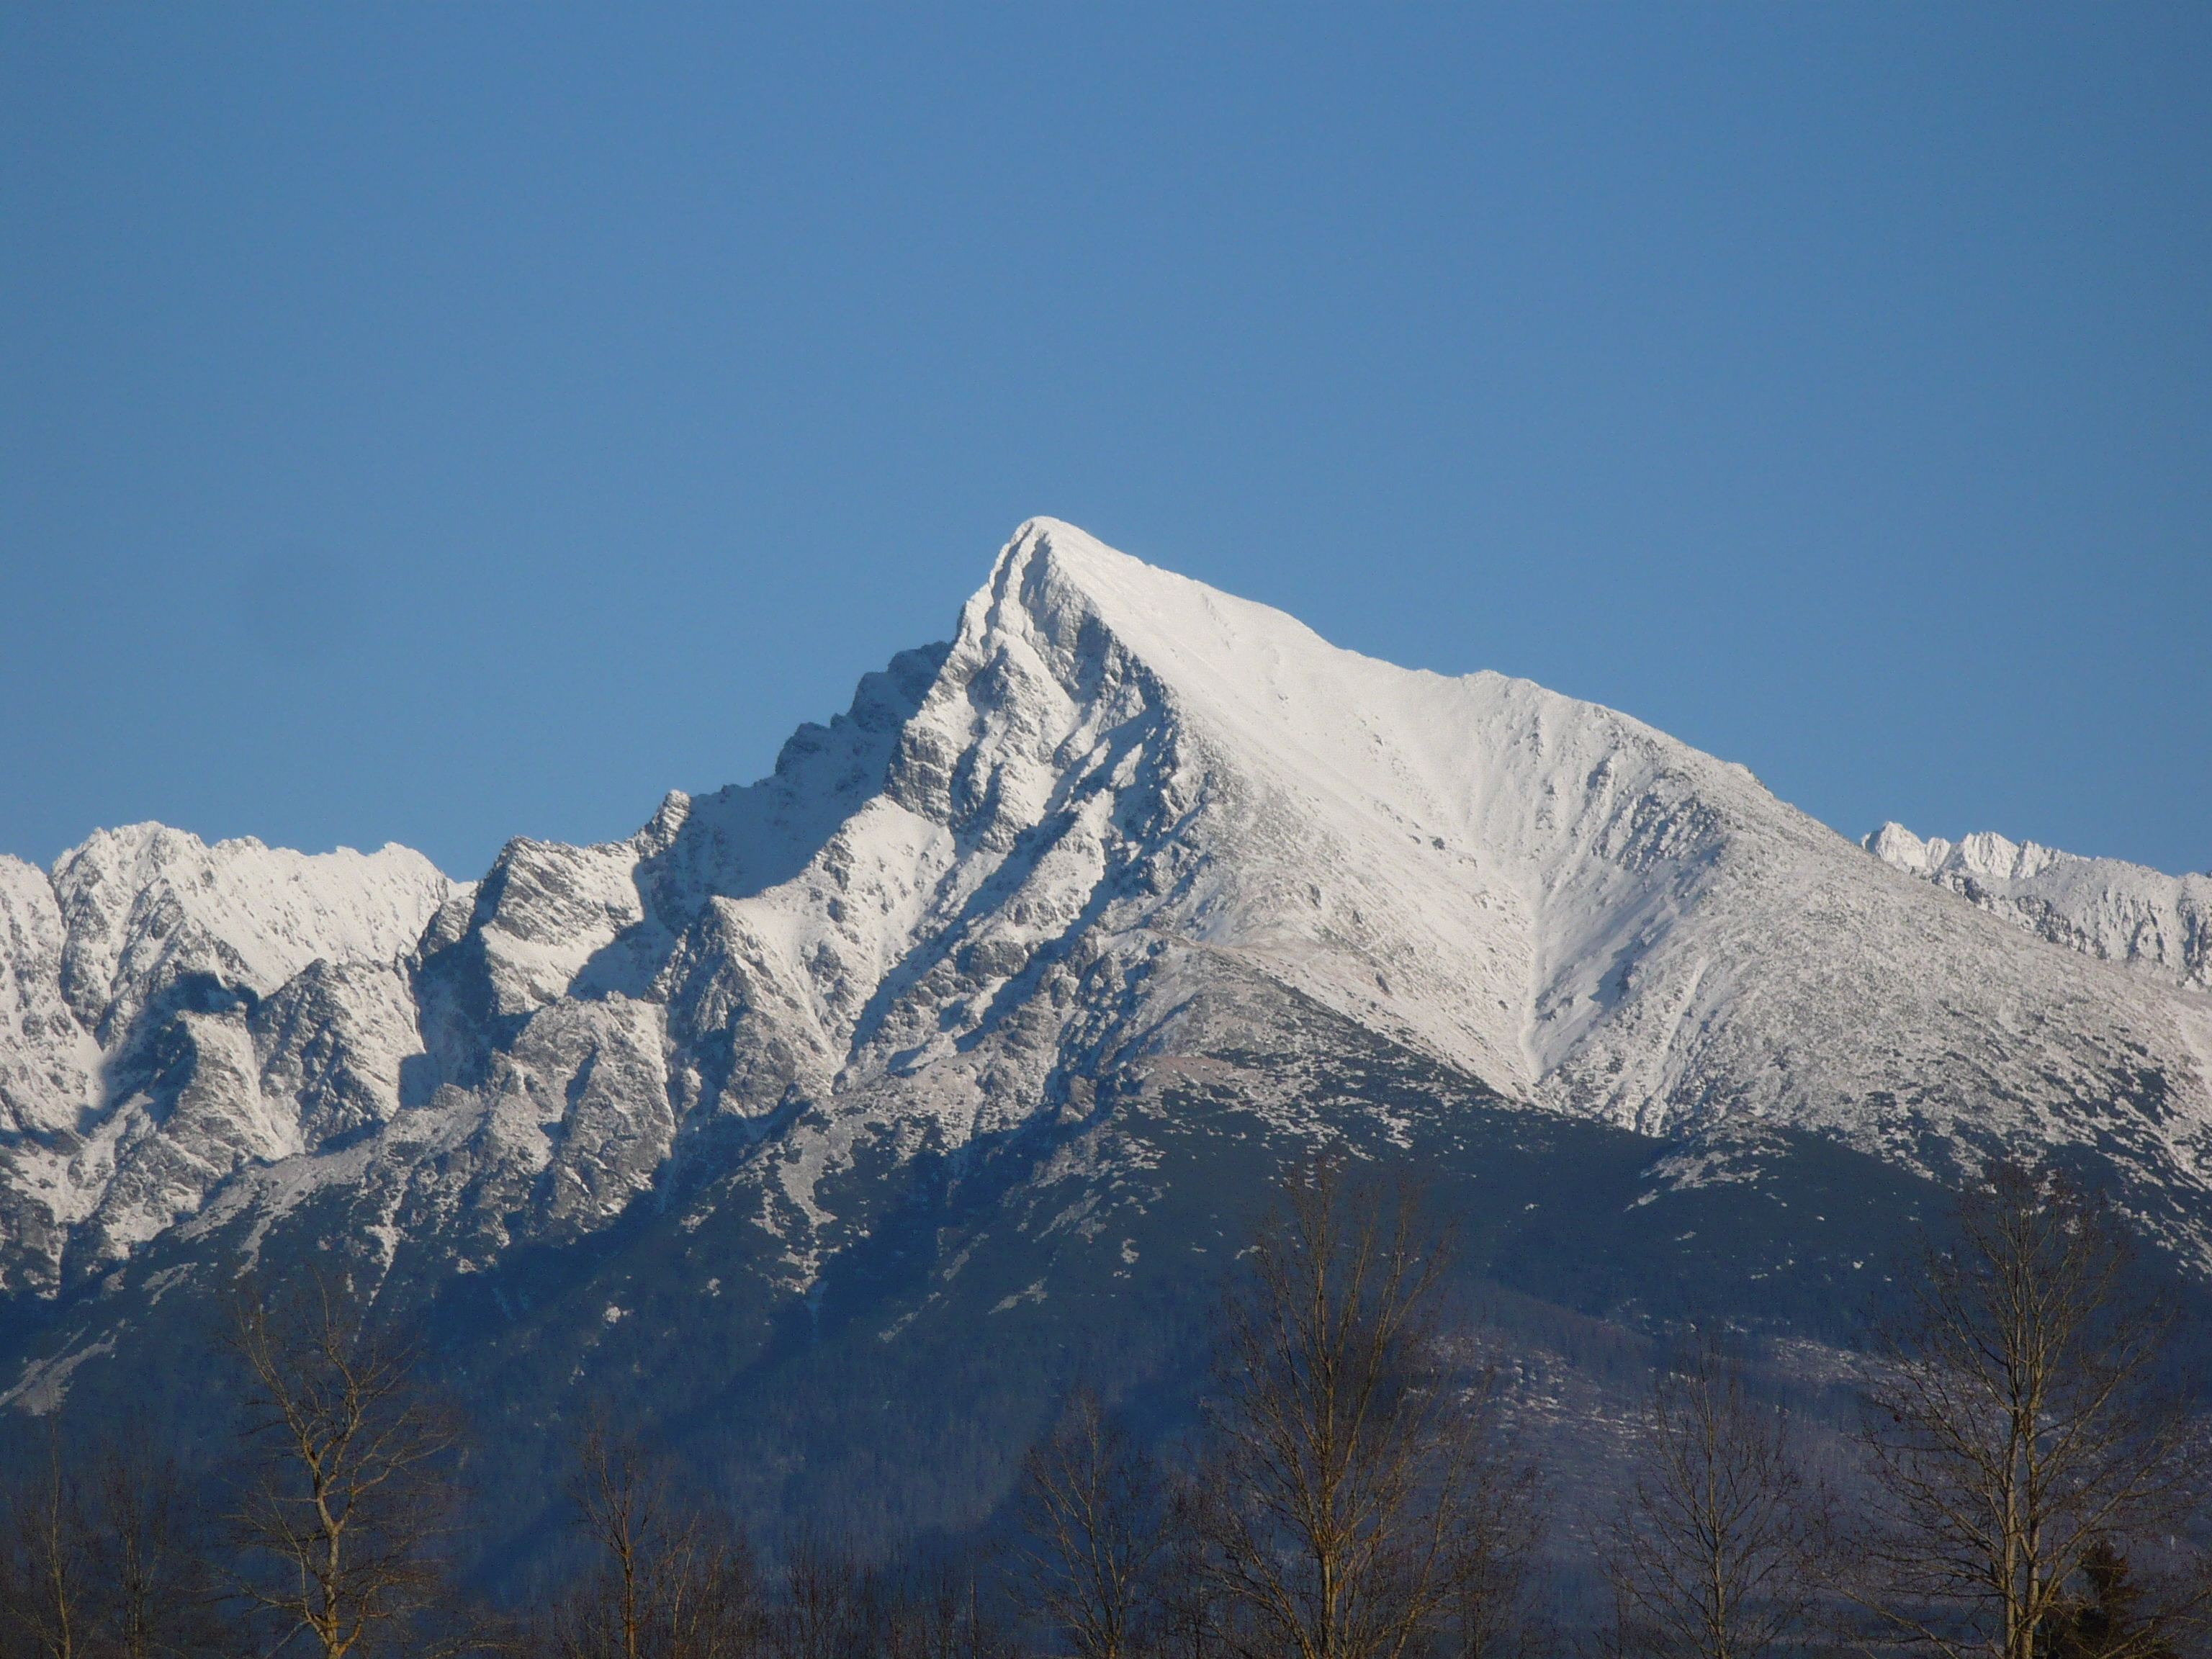
\includegraphics[width=1.\textwidth]{krivan}
\end{figure}

Obrázky \LaTeX\ vloží tam kde si je miesto a tam kde sa mu to hodí pomocou svojich pravidiel. My toto správanie môžeme ovplyniť pocmou argumentov figure a ich kombinácii. 
\begin{enumerate}
\item h - here, vlož obrázok približne sem
\item t - top, vlož obrázok na začiatok strany
\item b - bottom, spodok strany
\item p - page, vlož obrázok na špeciálnu stranu určenú pre plávajúce objekty (obrázky, tabuľky, ...)
\item ! - prinúť \LaTeX\ dať obrázok naozaj tam kde chcem
\item H - vlož obrázok tam kde je v kóde. Je potrebný float package
\end{enumerate}
Príklad použitia + k obrázkom sa dá pridať aj popis pomocou caption
\begin{figure}[H]
  \centering
      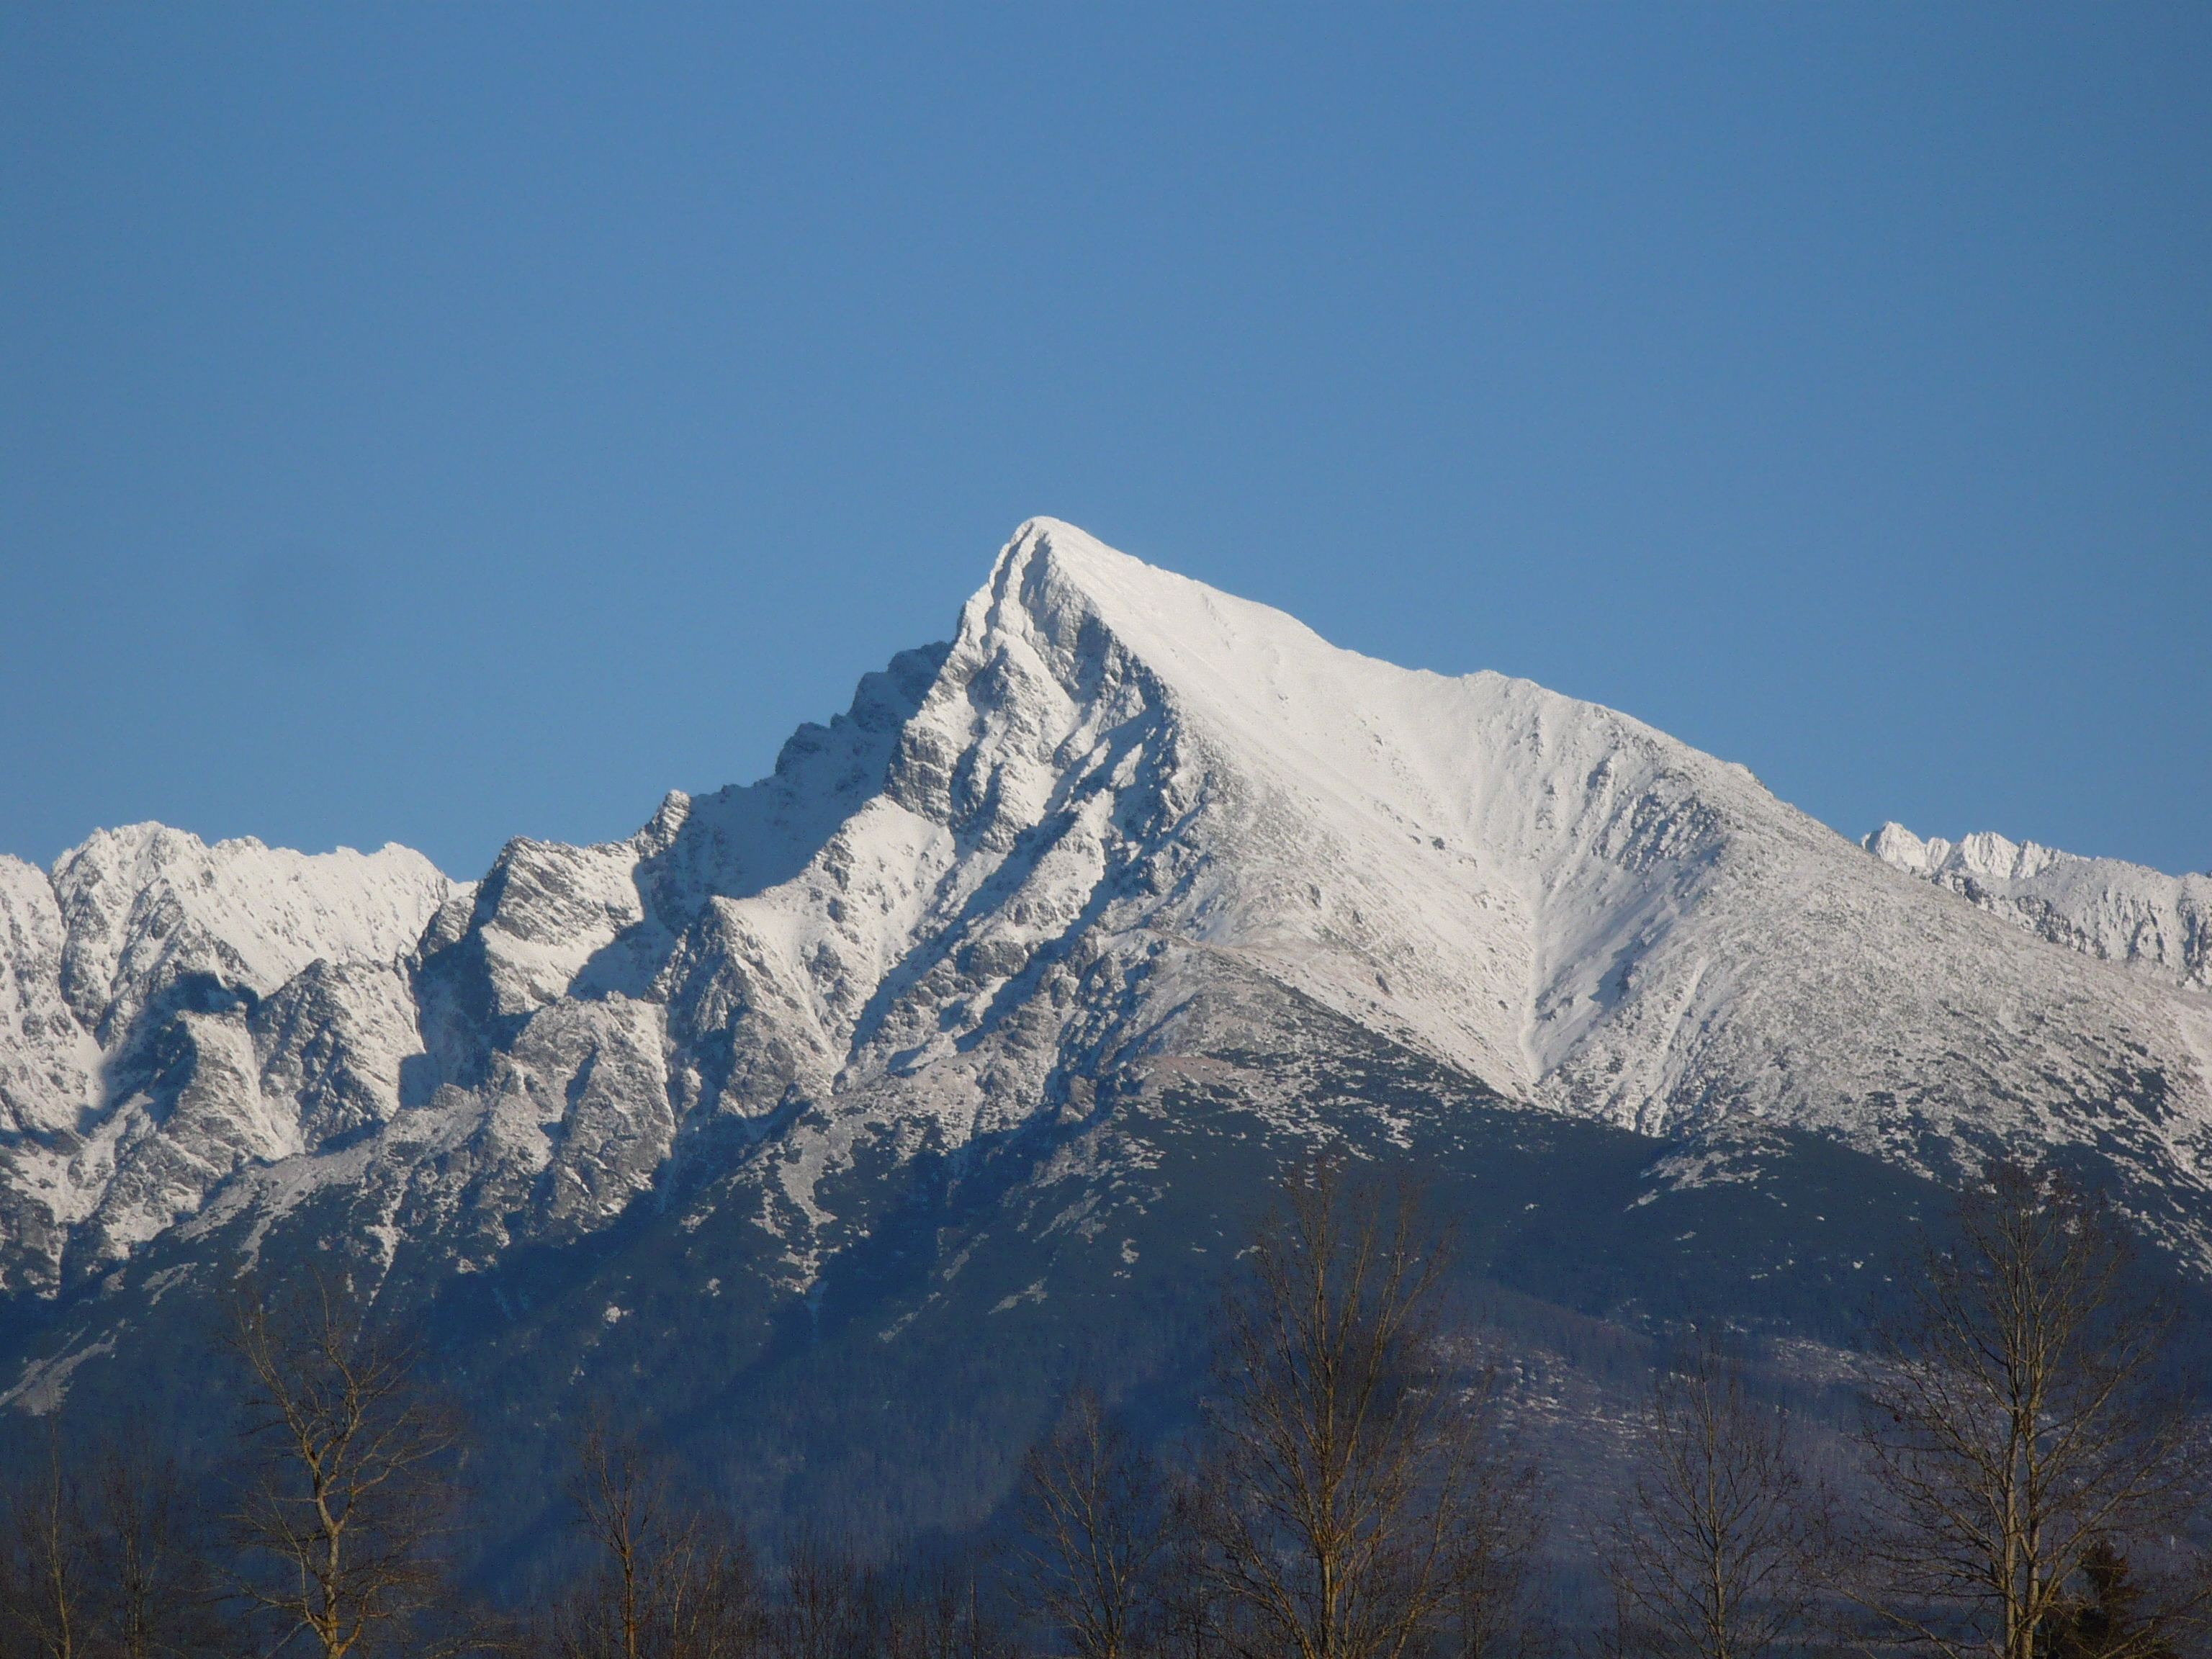
\includegraphics[width=0.5\textwidth]{krivan}
      \caption{Toto je popis k fotke Krivaňu. Je to taktiež prvý očíslovaný obrázok, kedže ako jediný ma popis}
\end{figure}

\clearpage
\newpage
\section{Referencie} \label{sec:referencie}
Každý vedecký článok by mal svoje zdroje referencovať. Ja som napríklad pri písaní tohto dokumentu použil viacero zdrojov, ktoré by som mal priznať. Mal by som ich priznať rovno vtedy, keď som ich použil ale pre učely tohto dokumentu ich budem referencovať až tu nakoniec.

Okrem iných prác by sme mali referencovať aj na svoje vlastné rovnice, obrázky, tabulky, sekcie atď. Keďže pridaním rovnice sa mi môže zmeniť číslovanie rovníc nemóžem napísať napr. viď rovnica 7 ale musím sa na odkazovať nejako inak. Nato slúži label. label sa dá pridať k rovniciam, obrázkom, tabulkám, sekciam a možno aj niekde inte. Pre sekciu viď label tejto sekcie. Pre rovnicu a obrázok viď nasledujúcu rovnicu a obrázok.
\begin{gather}
a_0=\frac{1}{\pi}\int\limits_{-\pi}^{\pi}f(x)\,\mathrm{d}x\\[6pt]
\begin{split}
a_n=\frac{1}{\pi}\int\limits_{-\pi}^{\pi}f(x)\cos nx\,\mathrm{d}x=\\
=\frac{1}{\pi}\int\limits_{-\pi}^{\pi}x^2\cos nx\,\mathrm{d}x
\end{split}\\[6pt]
\begin{split}
b_n=\frac{1}{\pi}\int\limits_{-\pi}^{\pi}f(x)\sin nx\,\mathrm{d}x=\\
=\frac{1}{\pi}\int\limits_{-\pi}^{\pi}x^2\sin nx\,\mathrm{d}x
\end{split} \label{eq:rovnica}
\end{gather}

\begin{figure}[H]
  \centering
      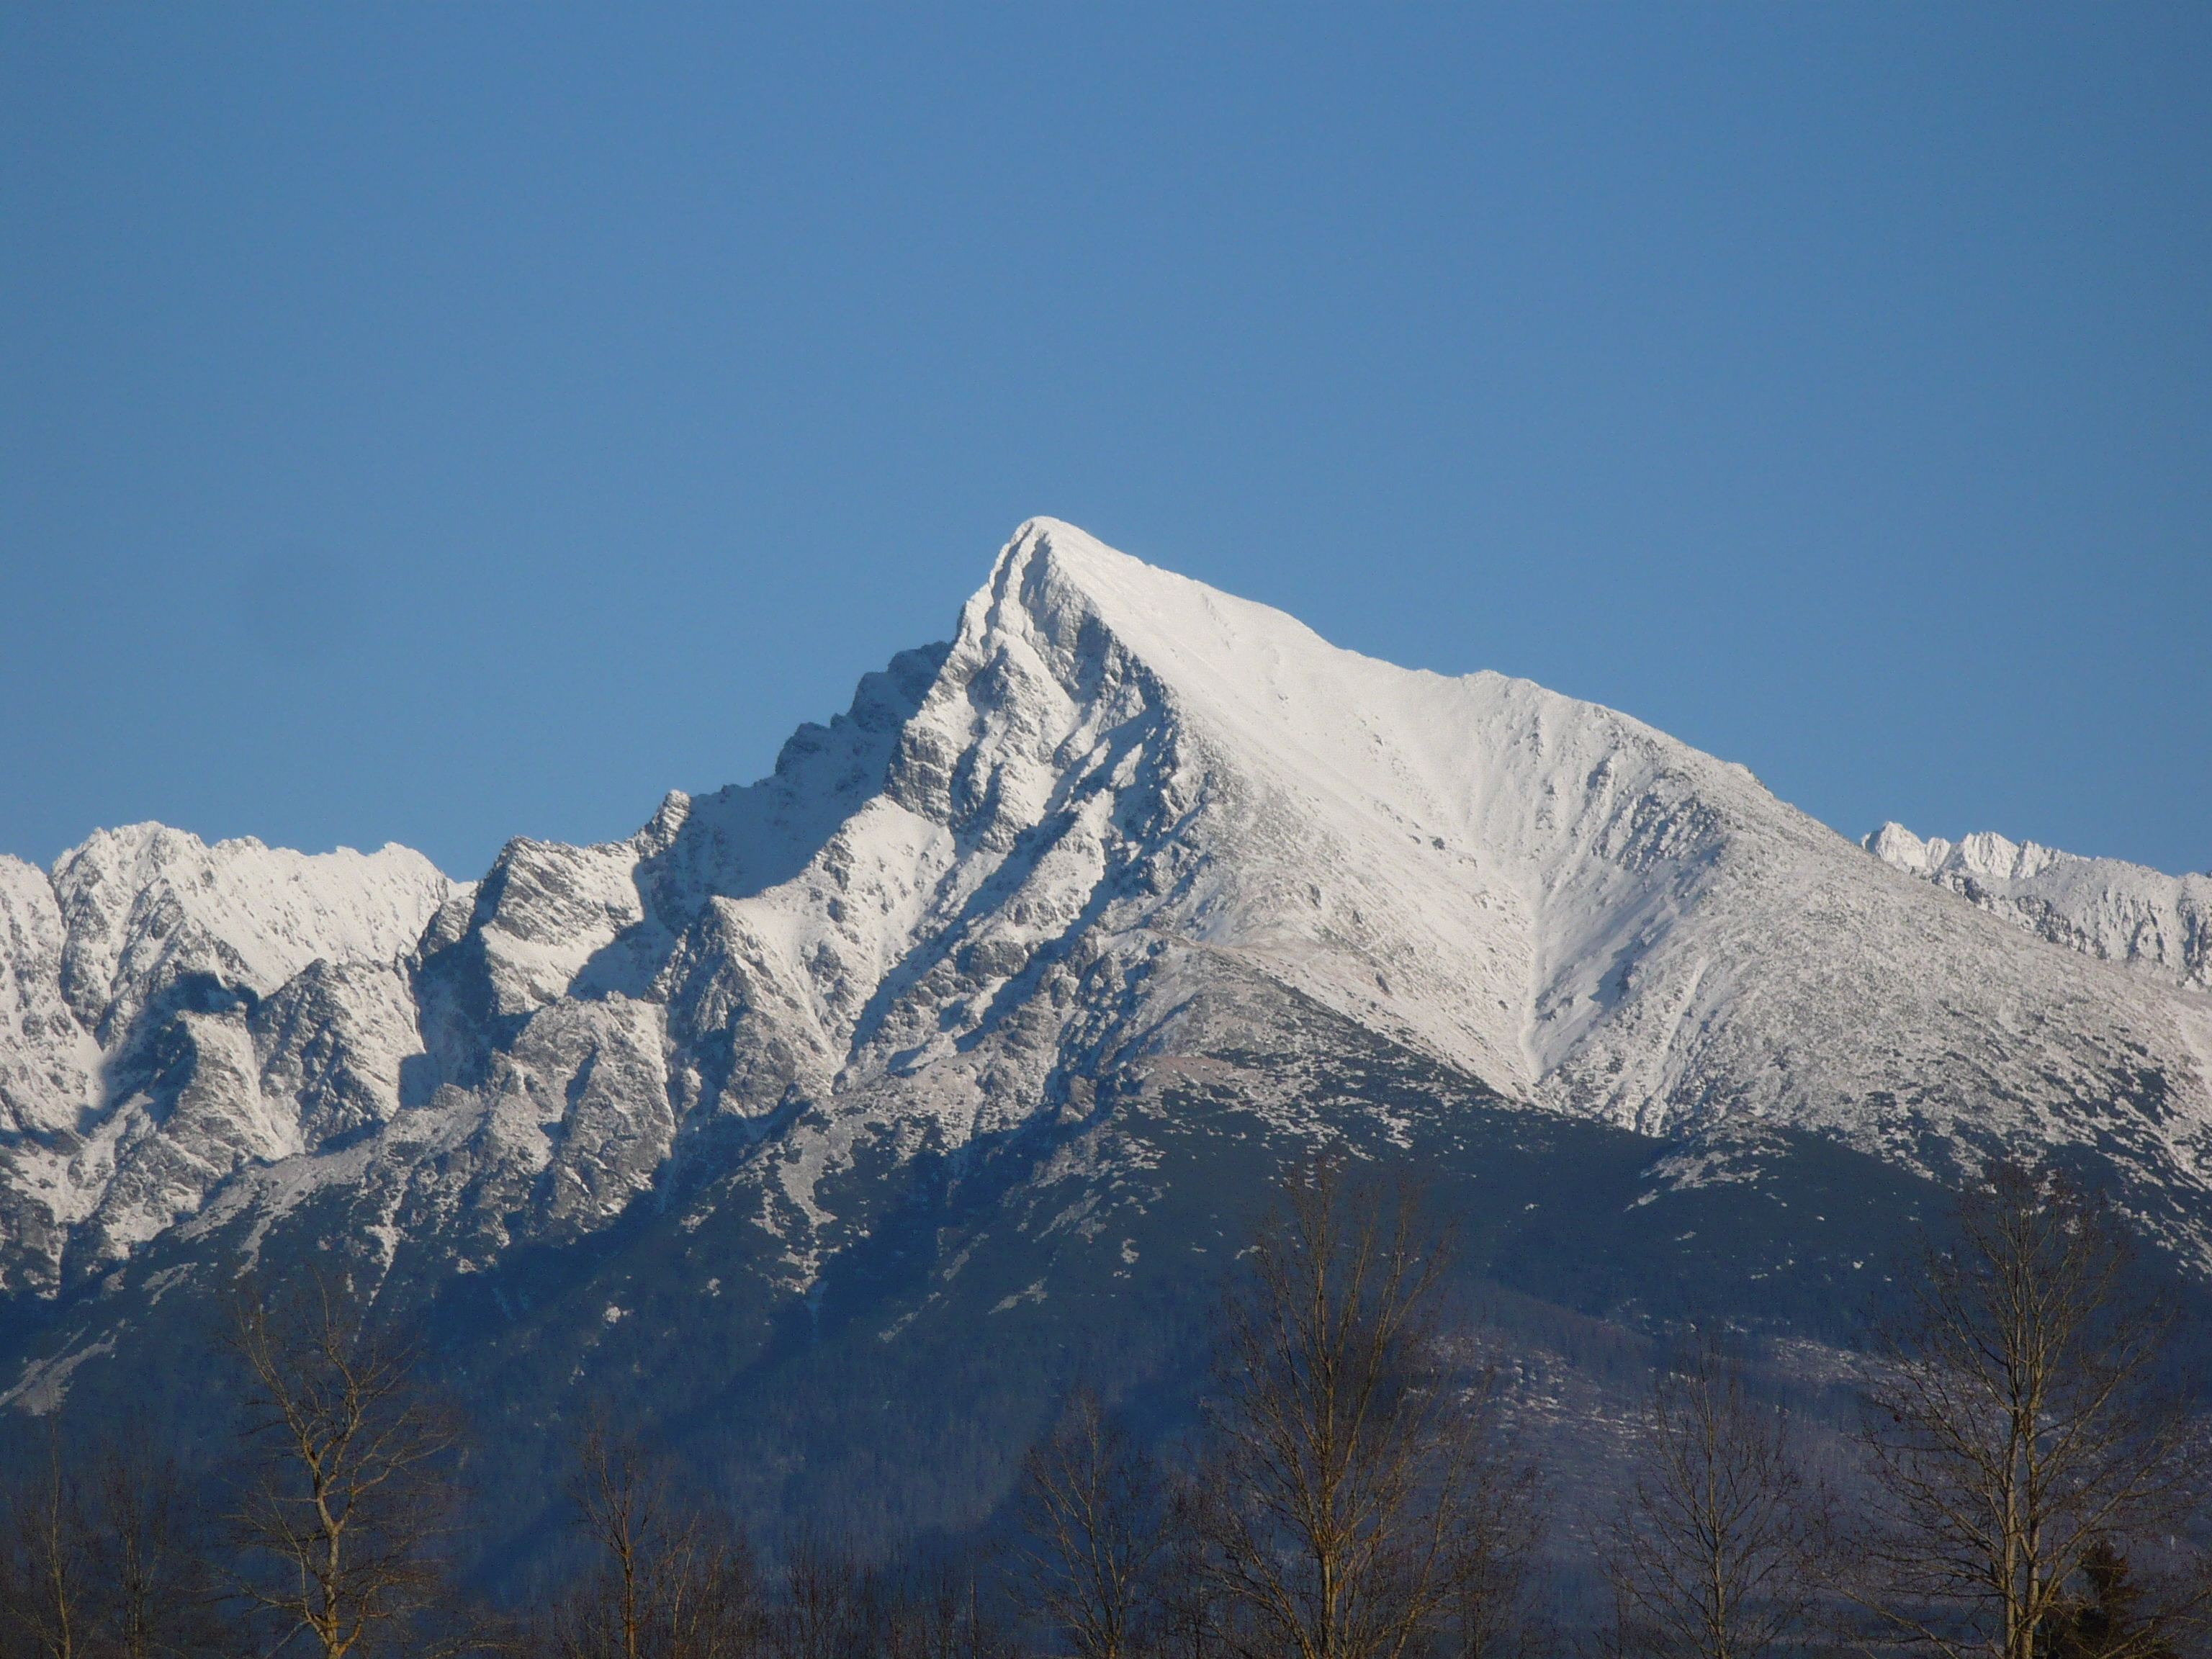
\includegraphics[width=0.7\textwidth]{krivan}
      \caption{Toto je fotka Kriváňu, na ktorú sa môžem odkazovat pocmocou jeho label \label{fig:krivan}}
\end{figure}

Rovnicu potom môžem referencovat pomocou ref. Napr. rovnicu (\ref{eq:rovnica}) v sekcii \ref{sec:referencie} som zobral zo stránky \url{https://en.wikibooks.org/wiki/LaTeX/Advanced_Mathematics}. Rovnice sa zvyknú dávať do () a referencie na zdroje do []. Obrázky sa referencujú len ako Obr. \ref{fig:krivan}.

Pri písaní tohto dokumentu som sa inšpiroval zdrojmi uvedenými v bibliografii. A možem na ne referencovať pomocou cite a názvu co je v bibitem. Napríklad v \cite{ShareLaTeX}. Zátvorky pridáva \LaTeX\ automaticky. Občas sa stane, že namiesto čísla je vo výslednom pdf dokumente v zátvorkách otáznik. Vtedy stáčí stlačiť preklad ešte raz alebo taký zdroj nemáte.

Písanie zdrojov má tiež svoje pravidlá. Píšu sa v abecednom poradí. Píše sa najkôr autor. Potom názov štýlom italic. Potom kde to bolo publikované a nakoniec rok. Môže sa to však líšit v závislosti od časopisu. Vo vašom prípade spôsob písania zdrojov určuje univerzita/fakulta. Tiež treba byť konzistentný v tom ako píšem mená autorov. Ak píšem celé meno tak ho treba písať celé všade. Ak píšem len iniciálky krstného mena, tak ho tak treba písať všade. Nasledujúca bibliografia je príklad ako sa to robiť nemá.

\begin{thebibliography}{9} %čislo 9 by malo určovať počet vecí v bibliografii. Načo to tam ale je, to neviem.
\bibitem{ShareLaTeX} 
Autor neznámy , \textit{ShareLaTeX guides}. 
\url{https://www.sharelatex.com/learn}.
 
\bibitem{prezentacia} 
RSI 2015 Staff, \textit{Introduction to \LaTeX}. Research Science Institute, Massachusetts Institute of Technology, \url{http://web.mit.edu/rsi/www/pdfs/new-latex.pdf}, 2015.

\bibitem{slovencina} 
Michal Szabados, \textit{Ako rozbehať slovenčinu v \LaTeX u}. \url{https://smnd.sk/mikey/download/utilitky/slovencina_v_LaTeXu.pdf}, 2008

\bibitem{slovnavod} 
Tobias Oetiker,Hubert Partl, Irene Hyna, Elisabeth Schlegl \textit{Nie príliš strucný úvod do systému \LaTeX\textnormal{2}$_\epsilon$}. \url{http://www.ptep-online.com/ctan/lshort_slovak.pdf}, 2002

\bibitem{spacing} 
K. Cooper, \textit{\LaTeX\ Spacing Tricks}. \url{http://www.math.wsu.edu/math/kcooper/M600/texspace.pdf}, 2012

\bibitem{equations} 
Stefan M. Moser, \textit{How to Typeset Equations in \LaTeX}. \url{http://moser-isi.ethz.ch/docs/typeset_equations.pdf}, 2016

\bibitem{uvod} 
Kubo, \textit{Úvod do \LaTeX u}. \url{https://people.ksp.sk/~kuko/tex/handouts/uvod.pdf}, 2005
\end{thebibliography}
\end{document}
